\section{Software Design}

The system was implemented using the Model-View-Controller (MVC) programming approach. The system does not strictly adhere to the MVC pattern, but uses it as a guideline to categorize the components of the system and its functionalities. Krasner and Pope \autocite{krasner-pope-88} discussed the benefit of using the MVC pattern to provide modularity by isolating functional components of the system, making it easier to design and modify.

\subsection{Business Layer}
 \label{subsection:controller}

 The business layer handles the internal logic of the application to solve the problem listed as the requirements of the system. In this particular case, the \emph{persistence layer} mentioned by Richards in \autocite{richards2015software} is combined with the business layer, as the logic of persisting necessary information on the database. By analyzing the use cases listed on \autoref{use_cases}, the functions of each component of the system can be defined, and consequentially a sequence of operations will be created for each specific use case. An additional sequence will also be defined as to complete the system and fulfill the requirements defined. 

\subsubsection{Customer Validation on a Registration Event}
 \label{subsection:regis}

\begin{figure}[!ht]
  \centering
  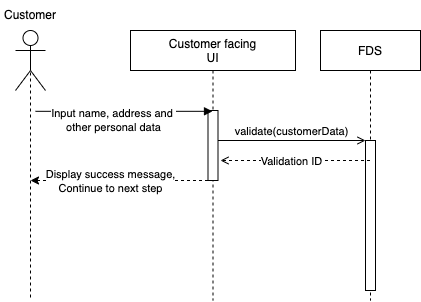
\includegraphics[width=0.6\textwidth]{diagrams/sequence-registration.png}
  \caption{System sequence diagram for a customer validation when a new customer is registered}
  \label{fig:regis-sequence}
\end{figure}

A system sequence can be defined by analyzing the following use case:

\begin{quotation}
 \enquote{As a stakeholder, I want to verify customer, so that the company can have more confidence that the existing user base is trustworthy} 
\end{quotation}

One of the opportunity to do a verification process is during a new customer registration. Verifying a customer after each new registration might help the stakeholder to be more confident, that the user base is trustworthy and necessary actions can be taken as soon as possible to reduce the possible damage made in the future by fraudulent customers. The following sequence will be executed as a way to validate a customer directly after a new registration:

\begin{itemize}
 \item A new customer inputs his or her personal data to a customer facing UI and clicks the \emph{"Register"} button
 \item The customer facing UI makes an HTTP Post request to the FDS, containing the user's personal data on its request payload
 \item The FDS receives the HTTP request, and schedules a new validation process to be executed asynchronously
 \item The FDS responds to the HTTP request by returning a validation ID pointing to the scheduled validation process
 \item Customer facing UI shows a success message and continues registration to the next step while the validation process runs 
\end{itemize}


\subsubsection{Notification on Suspicious Cases}
 \label{subsection:seq-notification}

\begin{figure}[!h]
 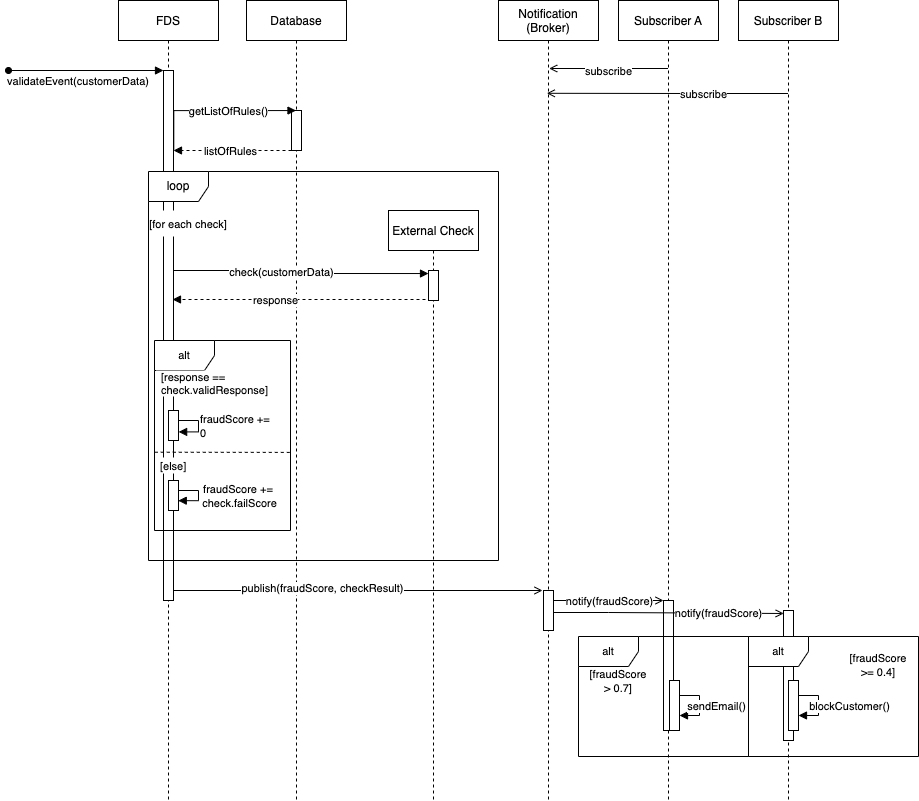
\includegraphics[width=\textwidth]{diagrams/sequence-notification.png}
 \caption{System sequence diagram for notifications on suspicious cases}
 \label{fig:notif-sequence}
\end{figure}

To fulfill the requirements of the system, a further examination of the following use case should be done:

\begin{quotation}
 \enquote{As an employee, I want to be notified when a user seems suspicious, so that I can do necessary actions accordingly} 
\end{quotation}

The FDS runs a rule evaluation by making an HTTP request to an external URL and comparing the HTTP response to the conditions listed on the validation rule. As working with external systems is unpredictable and there is no guarantee that the external system has a fast response time, a validation process is run asynchronously, meaning that the FDS would not return the validation result with a resulting fraud score directly to the client when a validation process is scheduled. At the end of a validation process, the concerned parties might need some kind of notification on certain cases, to make sure actions required can be made as soon as possible. The following sequence illustrates the sequence of activities done by the system to validate a certain customer and sending a notification on its completion:

\begin{itemize}
 \item The FDS receives an HTTP request to schedule a validation process and responds by returning the ID of the validation process
 \item FDS retrieves a list of validation rules from the database
 \item FDS begins to initiate a validation process by setting the fraud score to 0 and looping through the list of validation rules for evaluation
 \item A validation rule will be evaluated by making an HTTP request to the external endpoint defined by the validation rule and evaluating its response according to the condition specified
 \item If the response matches all the conditions specified by the validation rule, the rule evaluation will be considered as a success and the fraud score will be incremented with 0. Otherwise, the rule evaluation will be considered as a failure and the fraud score will be incremented by the \emph{fail score} specified by the validation rule
 \item After the evaluation of all validation rules retrieved from the database is completed, the FDS publishes the validation result to an exchange hosted by the message broker
 \item The message consumers consume the message from the exchange and react accordingly\footnote{For example: sending an email notification if the fraud score exceeds 0.7.}
\end{itemize}


\subsubsection{Managing Validation Rules}
 \label{subsection:management}

\begin{figure}[!ht]
  \centering
  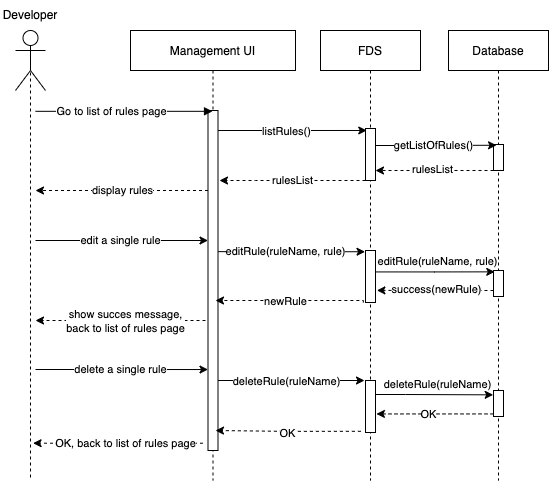
\includegraphics[width=0.8\textwidth]{diagrams/sequence-management.png}
  \caption{System sequence diagram for validation rules management}
  \label{fig:management_sequence}
\end{figure}

Another sequence can also be defined as a result of an analysis of the following use case:

\begin{quotation}
 \enquote{As an employee, I want to manage my own rule to validate users, so that I can use my expertise to find suspicious customers as efficiently as possible without the communication overhead with other teams} 
\end{quotation}

A possibility for each team to manage their own validation rules without being dependent to other teams is needed. By reducing the impediment in the process (having to consult other teams, communication overhead), every team can focus on generating validation rules that reflect a fraudulent customer as efficiently as possible, according to their own domain knowledge and expertise. The following sequence illustrates the functionality of managing validation rules:

\begin{itemize}
 \item A user (e.g. Developer) can access the management UI and go to the page that displays a list of available validation rules
 \item The FDS retrieves a list of validation rules from the database
 \item User can click on a single rule and edit the rule
 \item The management UI makes an HTTP PUT\footnote{In \autocite[\enquote{9.6 PUT}]{http-rfc}, HTTP PUT method is described as a method to store or modify an entity, defined by the Request-URI.} request to the database to edit an existing rule
 \item The FDS receives the HTTP request, modifies the rule on the database and returns the edited rule as a response
 \item The management UI displays a success message and redirects user back to the list of rules page
 \item User can click on a single rule and delete the rule
 \item The management UI makes an HTTP DELETE\footnote{In \autocite[\enquote{9.7 DELETE}]{http-rfc}, HTTP DELETE method is described as a method to delete a resource on the host server, pointed by the Request-URI.} request to the database to delete an existing rule
 \item The FDS receives the HTTP request and delete the rule on the database, returning a 204\footnote{In \autocite[\enquote{10.2.5 204 No Content}]{http-rfc}, the 204 status code should be used if the server fulfilled the request, but no data should be returned by the HTTP response.} status code as an identifier of a successful operation
 \item The management UI displays a success message and redirects user back to the list of rules page
\end{itemize} 


\subsubsection{Validation Real-Time Progress}

\begin{figure}[!ht]
 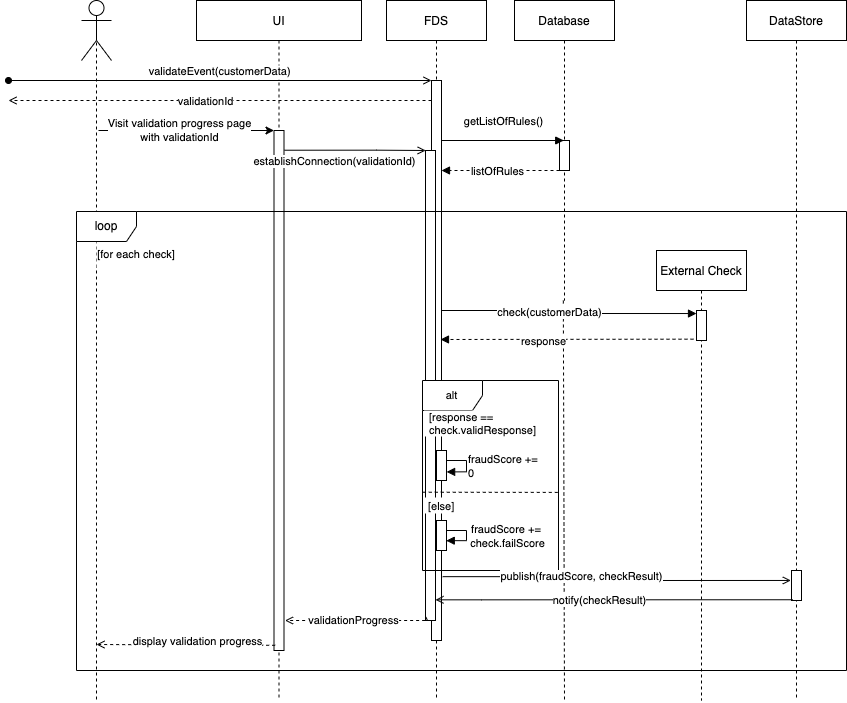
\includegraphics[width=\textwidth]{diagrams/sequence-pubsub.png}
 \caption{System sequence diagram for validation rules management}
\end{figure}

Even though the user should receive a notification on certain cases, there might be times when a user wants to intentionally monitor the progress of a validation process. To achieve such functionality, the user interface should establish a connection to the FDS, and receive notification whenever there is an update on the validation result. The sequence of such functionality will be as follows:

\begin{itemize}
 \item The FDS receives an HTTP request to schedule a validation process and responds by returning the ID of the validation process
 \item FDS retrieves a list of validation rules from the database and initiate the validation process
 \item A user visits the validation progress page with the returned validation ID
 \item The user interface establishes a connection with the FDS subscription endpoint
 \item After each rule evaluation, the FDS stores the latest validation result to a data store\footnote{A data store in this context can be a caching memory or a simple class to store some temporary information.}
 \item Every time the data store receives a new data, the user interface will get a notification and the latest result from the FDS subscription endpoint
 \item The user interface updates the view containing the latest validation result
\end{itemize}


\subsection{Model}
  \label{subsection:model}

As mentioned by Krasner and Pope \autocite{krasner-pope-88}, an application's model is a domain specific simulation or implementation of a structure. The model component of an MVC application contains business logic and manages the state of an application as well as its storage. 
The essential models of the system can be defined by revisiting the sequences listed on \autoref{section:sequence} and identifying the important structures needed to fulfill the requirements needed.
  
\subsubsection{Validation Rule}
A validation rule is a structure of information used in a validation process by supplying the FDS the necessary information to make an HTTP request to an external endpoint and evaluating its response, affecting the overall fraud score of a validation process through its evaluation result. Through a detailed analysis of the sequence listed on \autoref{subsection:seq-notification}, it is essential that the \emph{validation rule} model contains the following attributes:

\begin{itemize}
  \item A URL pointing to an external endpoint
  \item A list of conditions to evaluate the response returned by the external endpoint
  \item A unique identifier
  \item A fail score, which determine the severity of the rule if the evaluation failed
\end{itemize}

It might also be necessary to have an identifier in the validation rule to skip its evaluation in certain cases. Other than that, as the FDS would make an HTTP request to an external endpoint based on the information listed on a validation rule, the following attributes are needed to provide a more robust configuration:

\begin{itemize}
  \item HTTP method to be used to make the request
  \item Request header\footnote{In \autocite[\enquote{5.3 Request Header Fields}]{http-rfc}: request header is defined as additional information passed by the client to the host server about the particular request or about the client.}
  \item Request body
\end{itemize}

As the FDS interacts with external endpoints, there is no guarantee that the external endpoint will always be accessible. An additional attribute to specify and configure a retry strategy in such cases can be useful. However, a retry strategy can be really specific to its implementation and therefore will be discussed in \textbf{TODO: Add retry strategy implementation}.

An additional \emph{priority} attribute is also provided to enable the possibility to run rule validations according to its priority order.

\begin{figure}[!ht]
  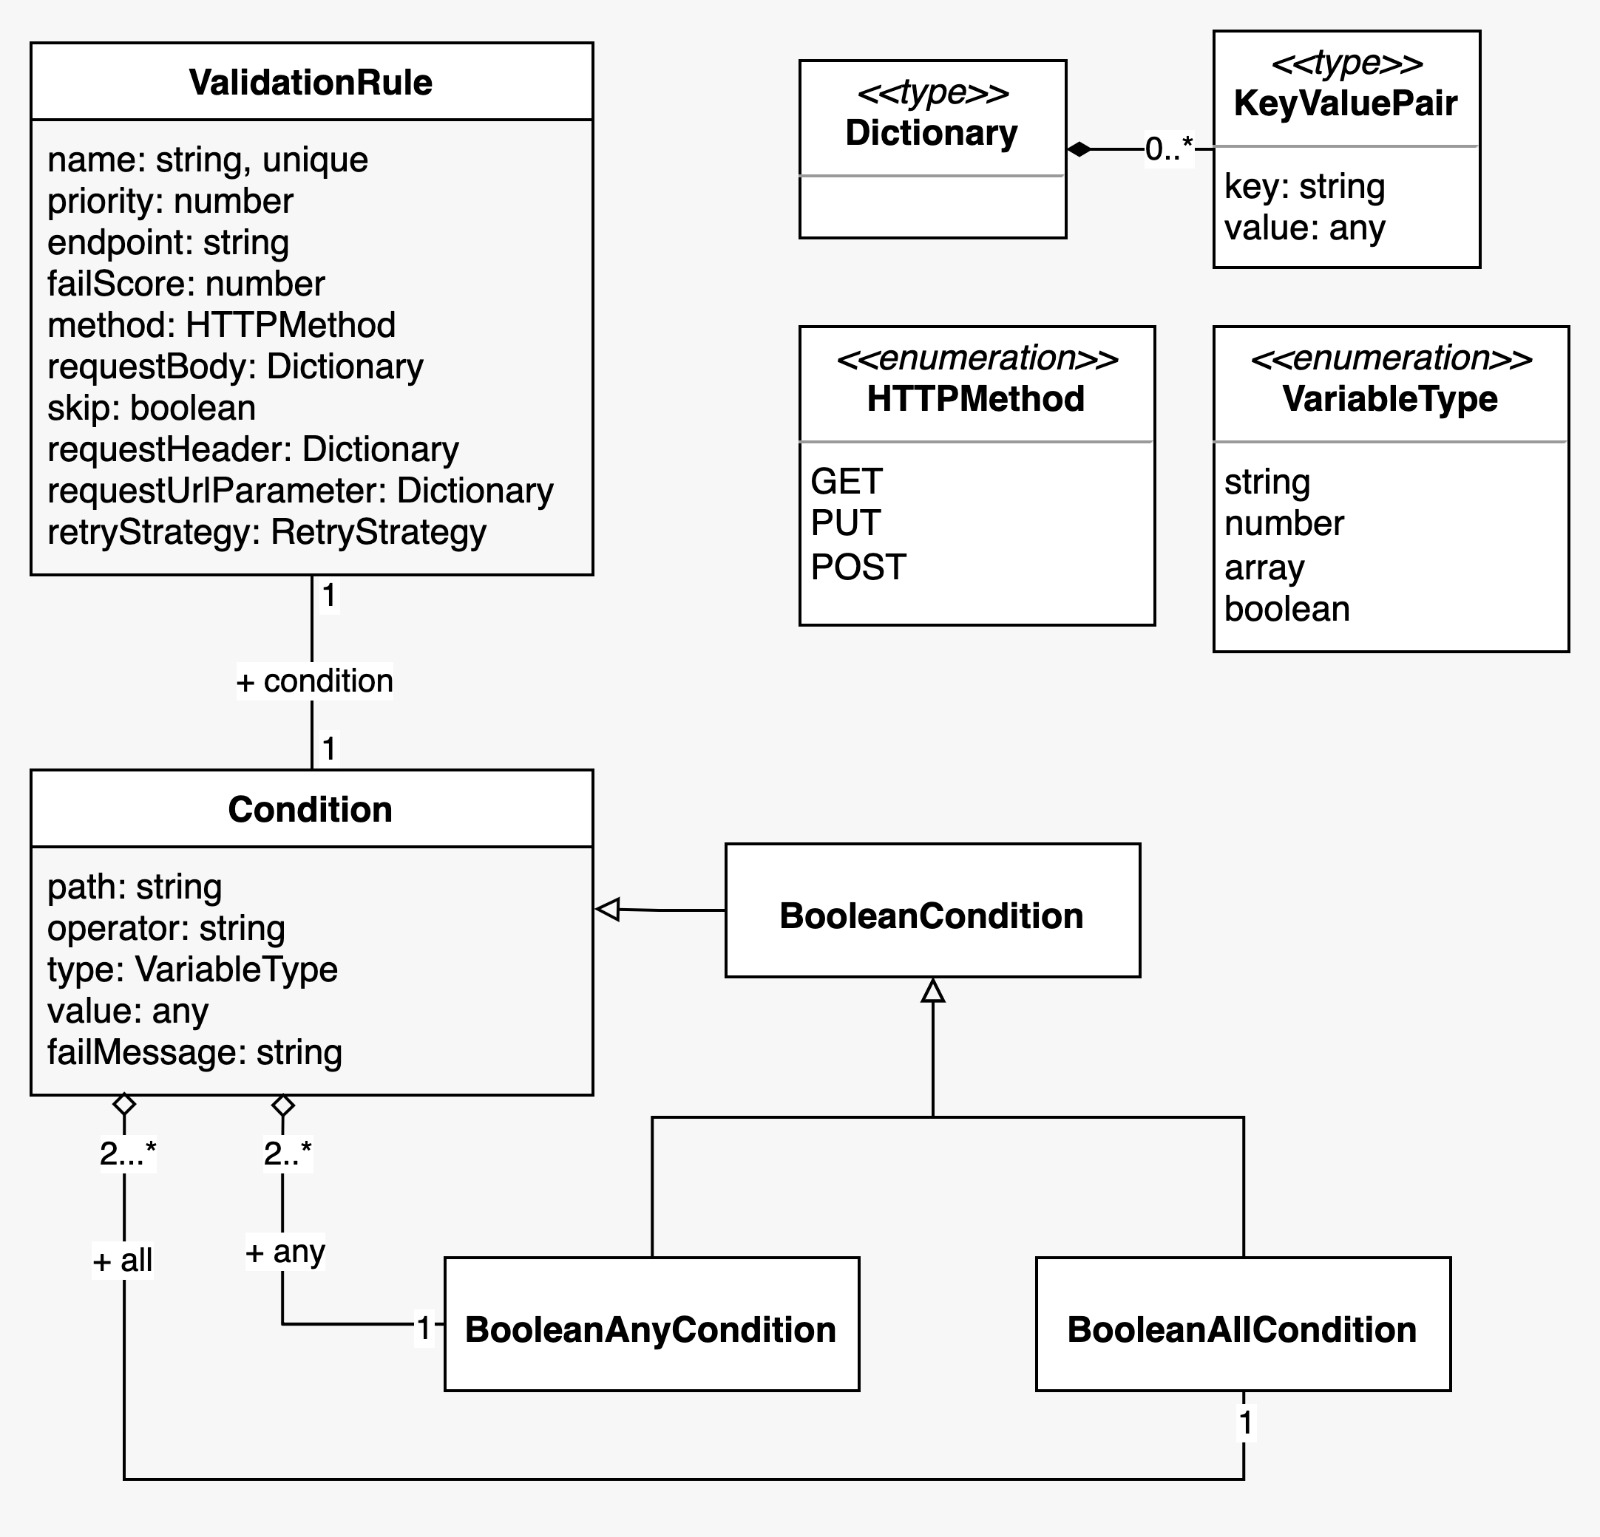
\includegraphics[width=\textwidth]{diagrams/entity_validation_rule.jpeg}
  \caption{UML diagram of the validation rule model}
 \end{figure}
 
The \emph{condition} attribute plays an important role for a validation rule, as it defines how the response returned by the external endpoint should be to pass a rule evaluation. It is intended to design the condition attribute to be robust and configurable. The \emph{path} of a condition defines a JSONPath\autocite{Friesen2019} expression to access information available of the current validation scope, such as customer information or response returned by the external endpoint. The \emph{type} attribute of a condition determines the type of the attribute accessed by the \emph{path} attribute. The \emph{type} attribute determines which type of operators are available to use\footnote{For example: a condition with \emph{type} "string" cannot use the "incl" \emph{operator}, because the "incl" \emph{operator} is only available for "array" \emph{type}}. The \emph{operator} attribute refers to a name of operator to be used to evaluate the condition (for example: "eq", "incl"). The available operator names are predefined and restricted to the condition's type attribute. More information regarding operators will be discussed in \textbf{TODO: Add retry strategy implementation}. The \emph{failMessage} attribute of a condition refers to a message that is going to be appended to the validation result's \emph{messages} attribute after a validation is completed.

\newpage
\begin{lstlisting}[caption={Validation rule example (JSON)}]
  {
    "name": "Example",
    "skip": false,
    "priority": 2,
    "endpoint": "http://localhost:8000/validate",
    "method": "GET",
    "failScore": 0.7,
    "condition": {
      "path": "$.response.statusCode",
      "type": "number",
      "operator": "eq",
      "value": 200,
      "failMessage": "Status code doesn't equal to 200"
    },
    "requestUrlParameter": {},
    "requestBody": {},
    "requestHeader": {}
  }
\end{lstlisting}

A validation rule might contain more than a single condition to pass an evaluation. In such cases, the user need to define whether how to determine whether an evaluation should pass: either pass an evaluation if \textbf{ALL} the conditions is true or pass an evaluation if \textbf{AT LEAST ONE (ANY)} of the conditions is true. This can be achieved by having the \emph{condition} attribute as an object with a single attribute, either \emph{all} or \emph{any} and an array of conditions as the attribute's value.

\begin{lstlisting}[caption={Validation rule example with ALL conditions (JSON)}]
  {
    "name": "Example",
    "skip": false,
    "priority": 2,
    "endpoint": "http://localhost:8000/validate",
    "method": "GET",
    "failScore": 0.7,
    "condition": {
      "all": [
        {
          "path": "$.response.statusCode",
          "type": "number",
          "operator": "eq",
          "value": 200,
          "failMessage": "Status code doesn't equal to 200"
        },
        {
          "path": "$.response.body.valid_address",
          "type": "boolean",
          "operator": "eq",
          "value": false,
          "failMessage": "Address is invalid"
        }
      ]
    },
    "requestUrlParameter": {},
    "requestBody": {},
    "requestHeader": {}
  }
\end{lstlisting}

\begin{lstlisting}[caption={Validation rule example with ANY conditions (JSON)}]
  {
    "name": "Example",
    "skip": false,
    "priority": 2,
    "endpoint": "http://localhost:8000/validate",
    "method": "GET",
    "failScore": 0.7,
    "condition": {
      "any": [
        {
          "path": "$.response.statusCode",
          "type": "number",
          "operator": "eq",
          "value": 200,
          "failMessage": "Status code doesn't equal to 200"
        },
        {
          "path": "$.response.body.valid_address",
          "type": "boolean",
          "operator": "eq",
          "value": false,
          "failMessage": "Address is invalid"
        }
      ]
    },
    "requestUrlParameter": {},
    "requestBody": {},
    "requestHeader": {}
  }
\end{lstlisting}

\subsubsection{Validation Result}
\newpage
\subsection{Presentation Layer}
  \label{sub:design_view}

The presentation layer is the interface for the user to interact with the system. The presentation layer will be implemented as a graphical user interface, and it is specifically designed to facilitate the functionalities described in \autoref{subsection:controller}. Several mock-ups are created to better visualize how the user interface should be structured using a UI design tool called Figma.  

\subsubsection{Rule Management Form}

\begin{figure}[!h]
  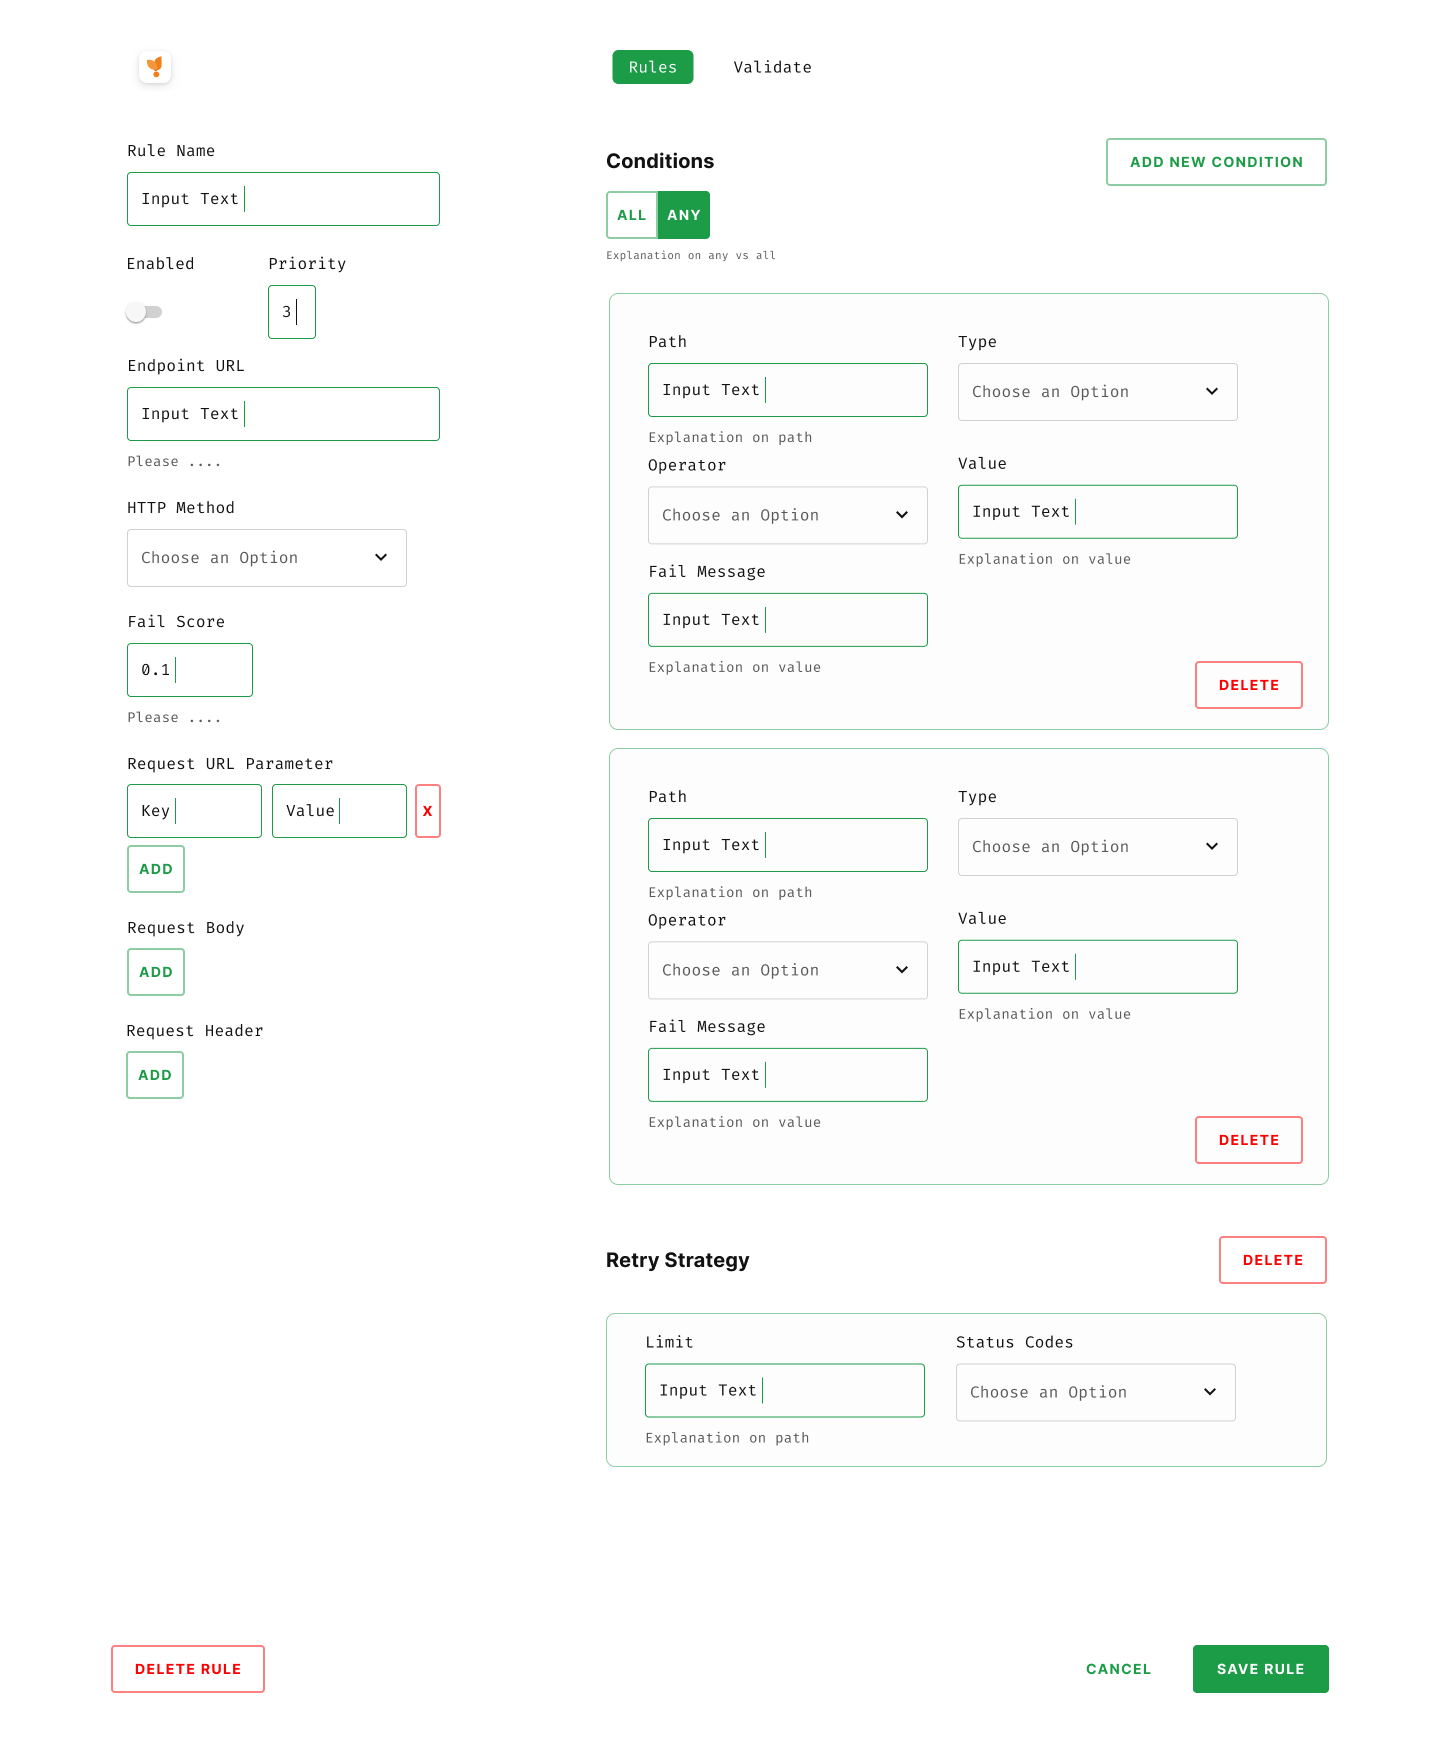
\includegraphics[width=\textwidth]{diagrams/mockup_rule_management.png}
  \caption{Mock up of the rule management form page}
\end{figure}

To facilitate the validation rule management functionality visualized in \autoref{fig:management_sequence}, a page containing a form to create, edit, delete and read a validation rule will be created. The rule management form is intended to be used by internal employee, preferably with technical background\footnote{An understanding on how HTTP works is a prerequisite to use the form.} to manage a validation rule that will be used to validate a customer.

The page should represent every attribute of a validation rule and gives the user the ability to modify the attribute if necessary. The form will be used both for rule creation and rule modification. For a rule creation, the form fields will be left blank. For a rule modification, the form fields will be filled with the rule's current data. 

The \textsc{Rule Name} field is used to display or enter a unique name of the validation rule. If the form is used to modify an existing rule, the field should be disabled, as a validation rule's name cannot be modified. 

The \textsc{Conditions} section can be used to add one or more condition to a validation rule. The form fields of each condition includes a dedicated input field for each attribute of a condition, as described in \autoref{subsub:rule}. The \textsc{Type} and \textsc{Operator} form fields are a selectable field, meaning the user has to select one out of several choices provided. This is intended to restrict input from the user, preventing an invalid condition being submitted to the FDS\footnote{For example, on \emph{type} field, user can only choose on of the following: (number, string, array, boolean).}. User can also delete a condition if necessary by clicking the \textsc{Delete} button available on each condition segment. If more than one condition is present, a selectable button will be displayed to select whether the "any" or "all" condition will be used. 

As the \verb;retryStrategy; attribute of a validation rule is not required, it is possible to delete an existing retry strategy, by clicking on the \textsc{Delete} button available on the \textsc{Retry Strategy} section of the form. If no retry strategy is present, a button to add a new retry strategy and to display the \textsc{Limit} and \textsc{Status Codes} fields will be displayed.

According to the model of a validation rule, \verb;requestBody, requestHeader; and \verb;requestUrlParameter; should be a dictionary that could contain as many entries as possible. To mimic this functionality as a form field, the \textsc{Request Body, Request Header} and \textsc{Request URL Parameter} fields are a dynamic input field. A dynamic input field enables the user to add a new key-value pair to the dictionary by clicking on the \textsc{Add} button and inputting the values to the corresponding input fields. To delete an entry of a dictionary, a delete button is provided next to each key-value field. 

\subsubsection{Validation Form}

\begin{figure}[!h]
 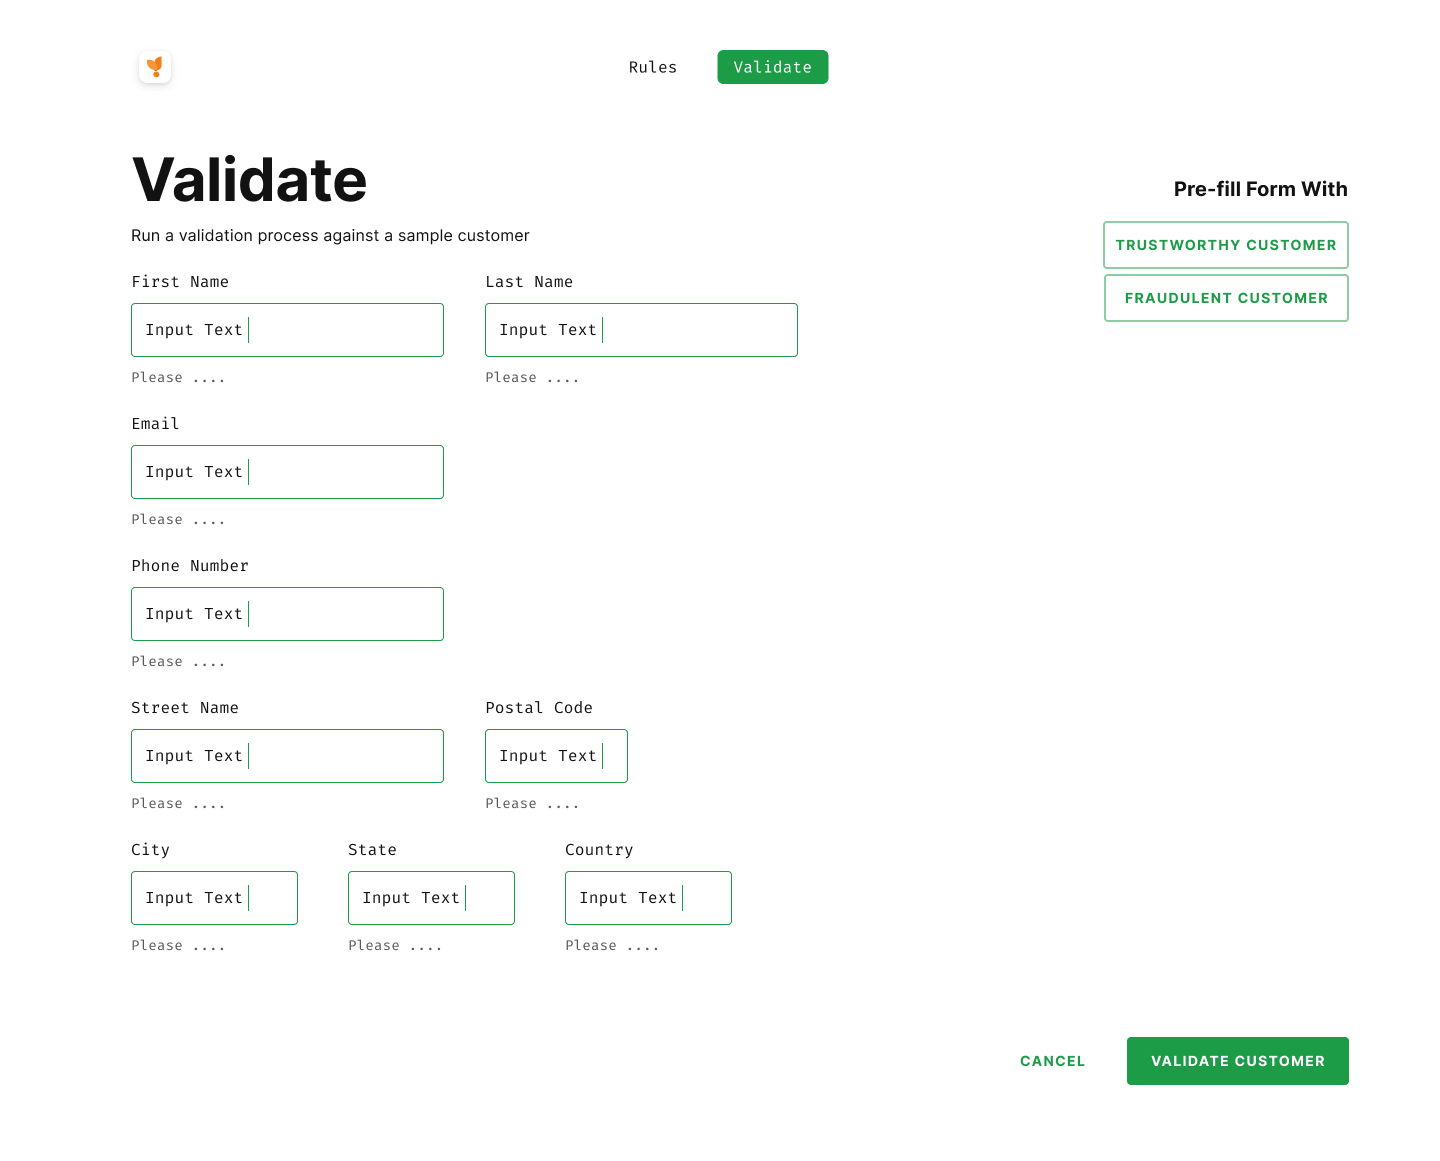
\includegraphics[width=\textwidth]{diagrams/mockup_validation_form.png}
 \caption{Mock up of the validation form page}
\end{figure}

A sample registration form is also created to give the user a possibility to run a validation process on a certain customer. The validation form is intended to be used by end customer, as a mean to register his-/herself into the system. Internal employees can also use the validation form to test the validation rules.

The page should represent a customer model by displaying every attribute of a customer in a form field (please refer to \autoref{fig:customer_uml} for more information on the customer model). For demonstration purposes, it might be beneficial to have a list of sample customers, so that the user can run a validation on a certain set of customers quickly, without having to first fill out the form by him-/herself. To provide this functionality, a list of buttons, containing a description text of the sample customer will be displayed next to the validation form. Upon clicking on one of the buttons, the validation form will be filled with the sample customer's data and the user can directly click on the \textsc{Validate Customer} button to begin the validation process.

\subsubsection{Validation Progress}

To provide a transparency on an asynchronous validation process, a page that displays the current progress of a validation process in real time might be beneficial. This page is intended for demonstration purposes, but can also be beneficial for security agents to keep track of the validation processes run by the FDS.

\begin{figure}[!h]
 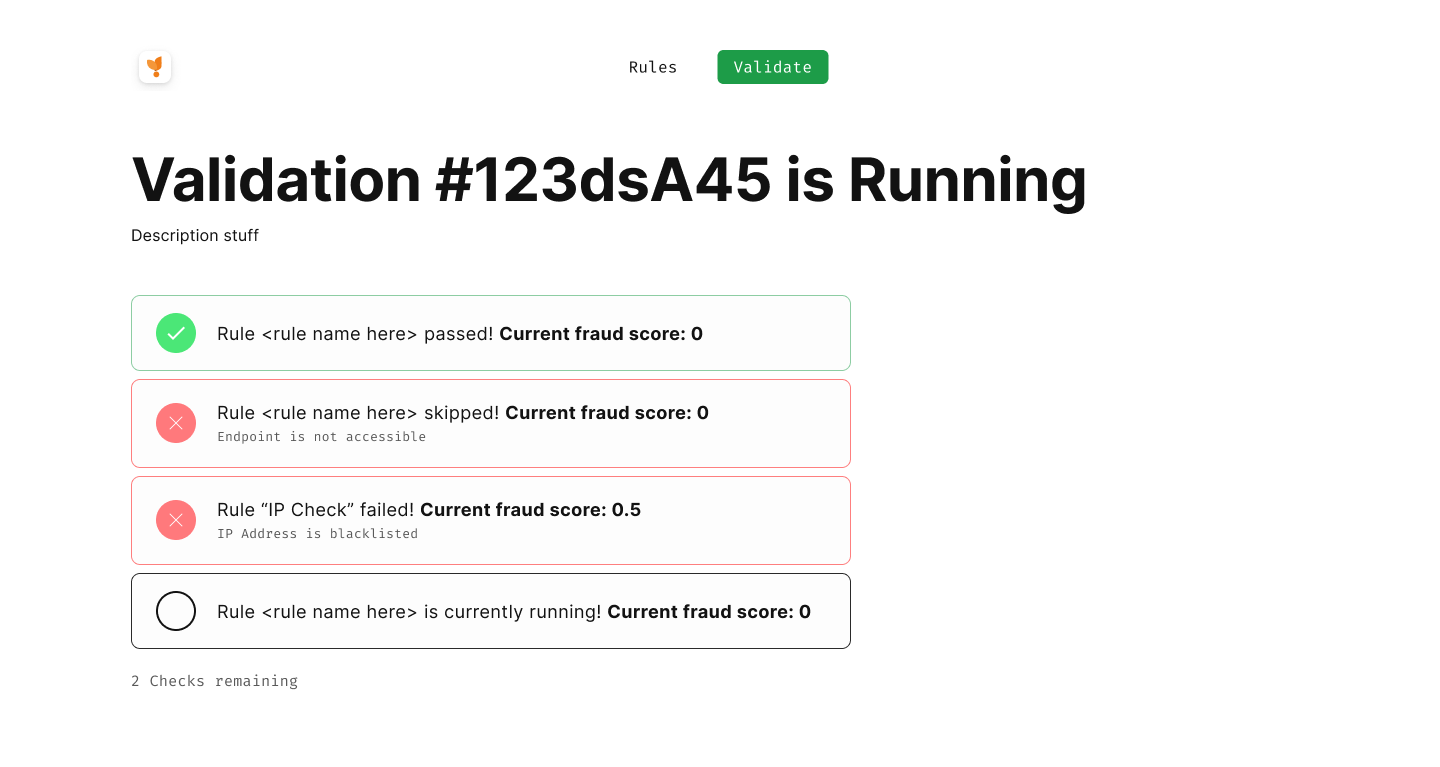
\includegraphics[width=\textwidth]{diagrams/mockup_validation_progress.png}
 \caption{Mock up of the validation progress page}
\end{figure}

The page displays the current progress of a certain validation in real time. It represents the \verb;events; attribute of a validation result in a timeline, displaying the events in a list. The page gives the user information regarding the evaluation result of each validation rule (success, failure, in progress or not started), the current fraud score and the names of validation rules that are skipped. If present, the messages of an event should also be displayed.  